% Springer Nature Article Template, version 3.1 (December 2024)
\documentclass[pdflatex,sn-mathphys-num]{sn-jnl}

\usepackage{graphicx}
\usepackage{amsmath,amssymb,amsfonts}
\usepackage{amsthm}
\usepackage{booktabs}
\usepackage{array}
\usepackage{url}
\usepackage{xcolor}
\hypersetup{
		pdftitle={ASTRAL: Auditable Structural Teacher Representation and Alignment Learning for Time-Series Classification},
		pdfauthor={Chen Deng and Han Zhang},
		pdfsubject={Interpretable representation learning for time-series classification},
		pdfkeywords={time-series classification, representation learning, structural similarity, kernel methods, interpretable machine learning}
}

\setlength{\emergencystretch}{2em}
\newcommand{\R}{\mathbb{R}}
\newcommand{\T}{\mathsf{T}}
\newcommand{\E}{\mathbb{E}}
\newcommand{\1}{\mathbf{1}}
\newcommand{\softmax}{\operatorname{softmax}}
\newcommand{\rank}{\operatorname{rank}}
\newcommand{\Std}{\operatorname{Std}}
\newcommand{\vecop}{\operatorname{vec}}
\newcommand{\RFFT}{\operatorname{RFFT}}
\newcommand{\SL}{\operatorname{SL1}}

\theoremstyle{plain}
\newtheorem{theorem}{Theorem}
\newtheorem{proposition}{Proposition}
\newtheorem{lemma}{Lemma}
\newtheorem{corollary}{Corollary}

\begin{document}

\title[ASTRAL for time-series classification]{ASTRAL: Auditable Structural Teacher Representation and Alignment Learning for Time-Series Classification}

\author[1]{\fnm{Chen} \sur{Deng}}\email{13260337317@163.com}
\author*[2]{\fnm{Han} \sur{Zhang}}\email{hanzhang@dufe.edu.cn}

\affil[1]{\orgdiv{College of Humanities and Communication},
  \orgname{Dongbei University of Finance and Economics},
  \orgaddress{\city{Dalian}, \state{Liaoning}, \country{China}}}
\affil*[2]{\orgdiv{School of Data Science and Artificial Intelligence},
  \orgname{Dongbei University of Finance and Economics},
  \orgaddress{\city{Dalian}, \state{Liaoning}, \country{China}}}

\abstract{Time-series representation models rarely expose the pairwise geometry that they learn. ASTRAL addresses this limitation with a deterministic, label-free teacher defined by multi-scale trend, residual-dynamics, and residual-spectrum descriptors. Their nonnegative kernel components sum to the teacher similarity, so every pair is associated with an exact three-part relation fingerprint. A retained kernel eigenspace provides a reference realization, while an inductive convolutional encoder approximates the same geometry using pairwise, Gram, neighborhood, component, and ordering losses. The encoder output is combined with standardized analytic features through dimension-based energy scaling. We prove positive semidefiniteness of the teacher kernel, conservation and local stability of the fingerprint, margin-based neighborhood preservation, correctness of the retained kernel coordinates, a truncation--amortization error bound, and properties of the hybrid feature space. On nine official UCR/UEA splits, the prespecified ten-method analysis gives ASTRAL 80.35\% unweighted mean accuracy and an average rank of 4.00. It exceeds its matched neural-only variant on all nine datasets by 4.23 percentage points on average. An additional frozen-protocol MultiROCKET run obtains 83.22\% mean accuracy but is not inserted retrospectively into the prespecified inferential family. The results support the proposed structural mechanism and its diagnostic value rather than general predictive superiority.}

\keywords{time-series classification, representation learning, structural similarity, kernel methods, interpretable machine learning}

\maketitle

	\section{Introduction}
	
	Time-series classification is fundamental to sensing, diagnosis, activity recognition, and industrial monitoring. Deep networks learn task-specific temporal representations, but the pairwise geometry encoded by those representations is difficult to inspect \cite{fawaz2019review}. Residual networks established a reproducible neural baseline \cite{wang2017scratch}, and InceptionTime demonstrated the value of multi-scale convolution and ensembling \cite{fawaz2020inceptiontime}. Random convolutional methods provide a complementary paradigm: ROCKET combines many random kernels with a linear classifier \cite{dempster2020rocket}, whereas MiniROCKET makes the transform almost deterministic and substantially faster \cite{dempster2021minirocket}. These methods are strong predictors, but their feature maps do not directly explain why a particular pair of series is similar.
	
	Predictive accuracy alone does not establish whether a representation captures meaningful and reproducible temporal structure. In explainable time-series classification, explanations should be connected to observable temporal evidence \cite{theissler2022xai}. When possible, inspectability should be built into the model rather than approximated by a separate post-hoc system \cite{rudin2019interpretable}. A representation-learning framework should therefore expose its target relation, component construction, realization error, and downstream utility as distinct, testable quantities.
	
	We introduce \textbf{ASTRAL}: \textbf{A}uditable \textbf{S}tructural \textbf{T}eacher \textbf{R}epresentation and \textbf{A}lignment \textbf{L}earning. ASTRAL defines a label-free similarity from multi-scale trend, residual dynamics, and residual spectrum; the three nonnegative components decompose every teacher relation exactly. ASTRAL-K realizes the centered teacher kernel in a retained eigenspace, and ASTRAL-N amortizes the same geometry with an inductive encoder. The deployed representation adds pooled shape and analytic descriptors under dimension-based energy scaling.
	
	The main contributions of this work are as follows:
	\begin{enumerate}
		\item A deterministic structural teacher whose similarity decomposes into nonnegative trend, residual-dynamics, and residual-spectrum contributions.
		\item Exact kernel coordinates and an inductive approximation of the same teacher, with separated spectral-truncation and neural-amortization errors.
		\item An energy-balanced hybrid representation combining learned coordinates, pooled morphology, and standardized analytic descriptors.
		\item Finite-sample guarantees and matched controls connecting kernel validity, attribution, approximation fidelity, fusion, and classification without assuming a class-optimal teacher.
	\end{enumerate}

	\section{Related Work}
	
	\subsection{Benchmarking and random convolutional classifiers}
	
	Large-scale archive evaluations have established dataset-level comparison as a standard protocol for time-series classification. The original bake-off systematically compared classifiers across heterogeneous datasets and emphasized ranks over isolated wins \cite{bagnall2017bakeoff}. The UCR archive subsequently consolidated a larger collection of univariate classification problems with predefined training and test splits \cite{dau2019ucr}. Comparable evaluation was extended to multivariate time series through the UEA archive and its associated bake-off \cite{ruiz2021uea}. More recently, the bake-off redux emphasized broader archive coverage, explicit dataset exclusions, reproducible implementations, and statistical comparison across datasets \cite{middlehurst2024redux}. These principles motivate our use of official splits, per-dataset results, average ranks, and dataset-level paired comparisons.
	
	Random convolutional transforms constitute particularly strong classification baselines. ROCKET applies a large collection of random convolutional kernels and summarizes their responses before fitting a linear classifier \cite{dempster2020rocket}. MiniROCKET removes most sources of randomness while retaining a high-dimensional convolutional feature map and substantially reducing computation \cite{dempster2021minirocket}. MultiROCKET extends this family through first-order differences and multiple pooling operators \cite{tan2022multirocket}. These methods motivate the random-convolution controls used below, although their feature maps are not designed to decompose an individual pairwise similarity.
	
	\subsection{Self-supervised representation and similarity learning}
	
	Self-supervised time-series methods obtain supervision from temporal structure, augmentations, masked observations, or relations among samples. Temporal Neighborhood Coding defines positive relations through local temporal neighborhoods \cite{tonekaboni2021tnc}. TS-TCC aligns weakly and strongly augmented views through temporal and contextual contrastive objectives \cite{eldele2021tstcc}. TS2Vec learns hierarchical contextual representations by contrasting representations across time steps and semantic scales \cite{yue2022ts2vec}. CoST separates seasonal and trend factors through contrastive objectives designed for disentangled forecasting representations \cite{woo2022cost}. TF-C couples time-domain and frequency-domain consistency during pre-training \cite{zhang2022tfc}, whereas SimMTM learns representations by reconstructing masked time series from neighboring observations in a learned manifold \cite{dong2023simmtm}. Patchwise independent embedding offers another route to transferable local representations by reducing dependence across time-series patches \cite{lee2024patches}. A broader taxonomy and review of these design choices is provided by Zhang et al. \cite{zhang2024sslreview}.
	
	The closest work to ASTRAL is Series2Vec, which uses temporal and spectral similarities as self-supervised targets for classification-oriented representation learning \cite{foumani2024series2vec}. Deep graph kernels have also been used to encode semantic relations between time-series subsequences \cite{yu2024deepgraph}. Differentiable elastic alignment, such as Soft-DTW, provides another mechanism for defining sequence-level relations \cite{cuturi2017softdtw}. ASTRAL differs in treating a prespecified signal relation as a common object for exact kernel realization, neural approximation, and component-wise inspection.
	
	\subsection{Relational transfer, kernel realization, and auditability}
	
	Relational knowledge distillation transfers relations among examples rather than relying only on pointwise output targets \cite{park2019rkd}. Similarity-preserving distillation similarly encourages a student network to reproduce a teacher's pairwise activation geometry \cite{tung2019spkd}. ASTRAL uses the same general principle, but its teacher is a deterministic function of signal descriptors rather than a pretrained label-aware model.
	
	Kernel methods provide the exact realization underlying this separation. Kernel PCA represents nonlinear sample geometry through the eigendecomposition of a centered Gram matrix \cite{scholkopf1998kpca}. ASTRAL-K applies this construction to the structural teacher kernel and retains the corresponding sample and out-of-sample coordinate maps. Kernel--target alignment measures agreement between a kernel and a supervised target matrix \cite{cristianini2002alignment}. In our protocol, this quantity is used only as a post-training audit on the training labels and does not participate in teacher construction, representation learning, model selection, or test-label evaluation.
	
	Low-rank kernel methods such as the Nystr\"om approximation reduce computation by approximating the full Gram matrix \cite{williams2001nystrom}. Our analysis instead distinguishes the spectral error from retaining finitely many teacher-kernel coordinates and the amortization error introduced by the inductive encoder.

	\section{ASTRAL Method}
	
	Let $x_i\in\mathbb{R}^{C_x\times L}$ denote the $i$th time series after independent per-series, per-channel standardization. All fitted statistics and model parameters use the official training split. Labels enter only through the final linear classifier; they do not construct descriptors, calibrate kernels, train the encoder, or select the pretraining epoch. Figure~\ref{fig:pipeline} summarizes the data flow.
	
	\begin{figure}[htbp]
		\centering
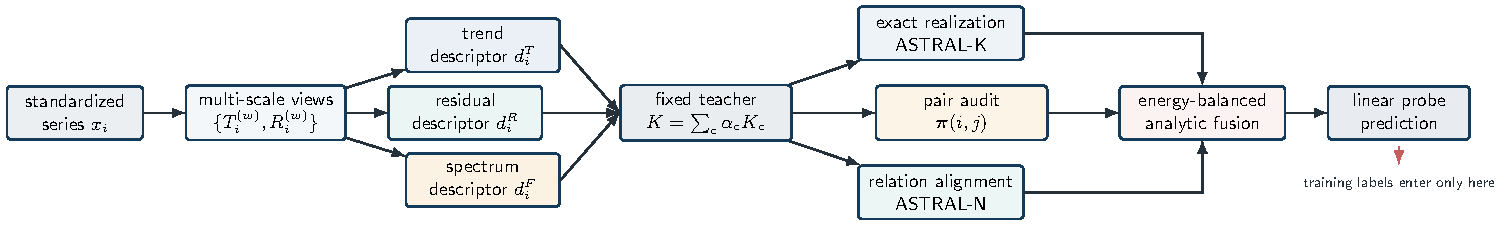
\includegraphics[width=0.98\linewidth]{Fig1_tikz.pdf}
		\caption{ASTRAL data flow. Descriptors define the teacher kernel; ASTRAL-K and ASTRAL-N provide spectral and inductive realizations, respectively. Training labels are restricted to the linear probe.}
		\label{fig:pipeline}
	\end{figure}
	
	\subsection{Multi-scale structural descriptors}
	
	The prescribed odd smoothing windows are $\mathcal{W}=\{5,11,25\}$. For requested window $w$ and series length $L$, the effective window is $\omega(w,L)=\min\{w,2\lfloor(L-1)/2\rfloor+1\}$; thus, an oversized window is replaced by the largest valid odd value. Replicate-padded moving averages define the trend and residual at scale $w$ as
	\begin{equation}
		T_i^{(w)}
		=
		\operatorname{MA}_{\omega(w,L)}(x_i),
		\qquad
		R_i^{(w)}
		=
		x_i-T_i^{(w)}.
		\label{eq:decomp}
	\end{equation}
	Both arrays retain the input length, and $x_i=T_i^{(w)}+R_i^{(w)}$ holds exactly at every scale.
	
	The neural path learns global logits $\{a_w:w\in\mathcal{W}\}$ and normalized weights $\beta_w=\exp(a_w)/\sum_{v\in\mathcal{W}}\exp(a_v)$. The aggregated trend and residual are
	\begin{equation}
		\overline{T}_i
		=
		\sum_{w\in\mathcal{W}}\beta_wT_i^{(w)},
		\qquad
		\overline{R}_i
		=
		x_i-\overline{T}_i.
		\label{eq:weighted}
	\end{equation}
	The weights satisfy $\beta_w\geq0$ and $\sum_w\beta_w=1$.
	
	For an array $y\in\mathbb{R}^{C_x\times q}$, let
	$\operatorname{Std}(y)$ denote independent channelwise centering and scaling,
	with a fixed denominator floor $\epsilon>0$. Let $P_m$ denote adaptive
	average pooling to $m=24$ positions, $\Delta$ the first-difference
	operator along time, and $\operatorname{vec}$ channel-preserving
	vectorization.
	
	The trend descriptor retains both level and first-difference summaries
	at all three scales:
	\begin{equation}
		d_i^{\mathrm{T}}
		=
		\operatorname{vec}\!\left(
		\left[
		P_m\!\left\{\operatorname{Std}\!\left(T_i^{(w)}\right)\right\};
		P_m\!\left\{\Delta\operatorname{Std}\!\left(T_i^{(w)}\right)\right\}
		\right]_{w\in\mathcal{W}}
		\right).
		\label{eq:trenddesc}
	\end{equation}
	
	Let $w^\star=\max_{w\in\mathcal{W}}\omega(w,L)$, $\widetilde r_i=R_i^{(w^\star)}$, and $r_i=\operatorname{Std}(\widetilde r_i)$.
	The raw residual $\widetilde r_i$ retains amplitude information, whereas
	$r_i$ is used for scale-normalized dependence and spectral summaries.
	For channel $c$ and lag $\ell$, define
	\begin{equation}
		\rho_{i,c}(\ell)
		=
		\frac{1}{L-\ell}
		\sum_{t=1}^{L-\ell}
		r_{i,c,t}\,r_{i,c,t+\ell},
		\qquad
		\ell=1,\ldots,q_a,
		\qquad
		q_a=12.
		\label{eq:acf}
	\end{equation}
	Writing $\rho_i(\ell)$ for the vector of channelwise autocorrelations,
	the residual descriptor is
	\begin{equation}
		d_i^{\mathrm{R}}
		=
		\operatorname{vec}\!\left(
		\left[
		\rho_i(1),\ldots,\rho_i(q_a);
		\mu_c(|r_i|);
		\sigma_c(\widetilde r_i);
		\sigma_c(\Delta\widetilde r_i)
		\right]
		\right),
		\label{eq:resdesc}
	\end{equation}
	where $\mu_c$ and $\sigma_c$ denote channelwise means and population
	standard deviations. Thus, the autocorrelation and absolute-deviation
	terms describe residual shape, while the last two terms retain residual
	amplitude and variation.
	
	For each channel, define the nonnegative log-amplitude spectrum $v_{i,c}=\log(1+|\operatorname{RFFT}(r_{i,c})|)$ and its normalized form $\widetilde v_{i,c}=v_{i,c}/(\|v_{i,c}\|_2+\epsilon)$. The frequency descriptor is
	\begin{equation}
		d_i^{\mathrm{F}}
		=
		\operatorname{vec}\!\left(
		\left[
		P_m\{\widetilde v_{i,c}\}
		\right]_{c=1}^{C_x}
		\right).
		\label{eq:freqdesc}
	\end{equation}
	
	The descriptor dimensions are
	\begin{equation}
		\begin{aligned}
			D_{\mathrm{T}}&=2|\mathcal{W}|C_xm,&
			D_{\mathrm{R}}&=C_x(q_a+3),&
			D_{\mathrm{F}}&=C_xm,\\
			D&=D_{\mathrm{T}}+D_{\mathrm{R}}+D_{\mathrm{F}}=183C_x.
		\end{aligned}
		\label{eq:dims}
	\end{equation}
	
	Because pooled structural summaries may suppress local morphology,
	ASTRAL additionally protects a direct shape sketch:
	\begin{equation}
		s_i
		=
		\operatorname{vec}(P_mx_i),
		\qquad
		a_i
		=
		\left[
		d_i^{\mathrm{T}};
		d_i^{\mathrm{R}};
		d_i^{\mathrm{F}};
		s_i
		\right]
		\in\mathbb{R}^{D_A},
		\qquad
		D_A=207C_x.
		\label{eq:analytic}
	\end{equation}
	The shape sketch is excluded from the structural teacher and is used
	only in the final analytic block.
	
	\subsection{Fixed teacher and conserved relation fingerprint}
	
	For each component $c\in\{\mathrm{T},\mathrm{R},\mathrm{F}\}$, let $\mathcal{Q}$ contain at most 1,024 distinct, non-self training
	pairs selected using the prespecified calibration seed. If fewer than
	1,024 such pairs are available, all distinct pairs are used. Define $\Delta_c^+=\{\|d_i^c-d_j^c\|_2:(i,j)\in\mathcal{Q},\ \|d_i^c-d_j^c\|_2>0\}$. The component scale is defined for ordinary and degenerate samples by
	\begin{equation}
		\tau_c=
		\begin{cases}
			\max\!\left\{10^{-6},\operatorname{median}(\Delta_c^+)\right\},
			& \Delta_c^+\neq\varnothing,\\
			10^{-6}, & \Delta_c^+=\varnothing.
		\end{cases}
		\label{eq:kernelscale}
	\end{equation}
	The sampled pair indices and resulting scales are fixed after
	calibration and reused for all test cases.
	
	The component kernels are Laplacian kernels on their respective
	descriptor spaces:
	\begin{equation}
		k_c(i,j)
		=
		\exp\!\left(
		-\frac{\|d_i^c-d_j^c\|_2}{\tau_c}
		\right).
		\label{eq:componentkernel}
	\end{equation}
	Their weighted sum defines the structural teacher:
	\begin{equation}
		k(i,j)
		=
		\sum_{c\in\{\mathrm{T},\mathrm{R},\mathrm{F}\}}
		\alpha_ck_c(i,j),
		\qquad
		(\alpha_{\mathrm{T}},\alpha_{\mathrm{R}},\alpha_{\mathrm{F}})
		=
		(0.4,0.3,0.3).
		\label{eq:jointkernel}
	\end{equation}
	Because every $\alpha_c$ is nonnegative and the weights sum to one,
	$k(i,i)=1$ and $0<k(i,j)\leq1$.
	
	For every pair $(i,j)$, the normalized component contribution is
	\begin{equation}
		\pi_c(i,j)
		=
		\frac{\alpha_ck_c(i,j)}{k(i,j)}.
		\label{eq:fingerprint}
	\end{equation}
	These contributions satisfy
	\begin{equation}
		\pi_c(i,j)\geq0,
		\qquad
		\sum_c\pi_c(i,j)=1,
		\qquad
		\alpha_ck_c(i,j)=\pi_c(i,j)k(i,j).
		\label{eq:fingerprint_conservation}
	\end{equation}
	Thus, $\boldsymbol{\pi}(i,j)=[\pi_{\mathrm{T}}(i,j),\pi_{\mathrm{R}}(i,j),\pi_{\mathrm{F}}(i,j)]$ is an exact pair-level relation fingerprint. It is not a post-hoc
	explanation of a classifier prediction; it is an algebraic
	decomposition of the teacher relation used during representation
	learning. Figure~\ref{fig:fingerprint} distinguishes the absolute
	weighted contributions from their normalized composition.
	
	\begin{figure}[htbp]
		\centering
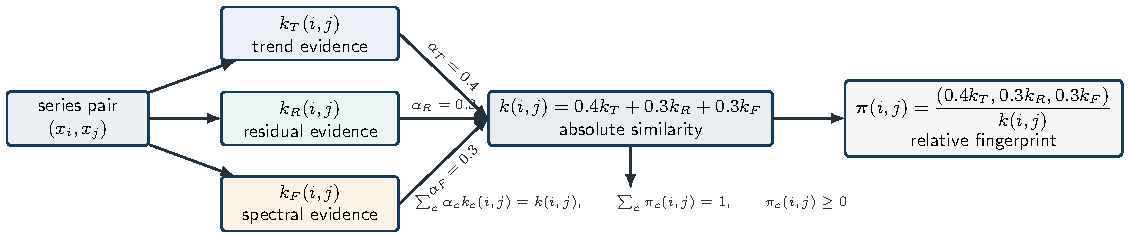
\includegraphics[width=0.98\linewidth]{Fig2_tikz.pdf}
		\caption{Decomposition of one teacher relation. Weighted component similarities sum to $k(i,j)$, and $\boldsymbol{\pi}(i,j)$ gives their normalized proportions.}
		\label{fig:fingerprint}
	\end{figure}
	
	\subsection{Exact kernel realization}
	
	Let $K\in\mathbb{R}^{n\times n}$, with $K_{ij}=k(i,j)$, be the teacher Gram matrix on the official training split. Define
	\begin{equation}
		H_n
		=
		I_n-\frac{1}{n}\mathbf{1}\mathbf{1}^{\top},
		\qquad
		K^\circ
		=
		H_nKH_n.
		\label{eq:centeredkernel}
	\end{equation}
	Let $K^\circ=U\Lambda U^\top$ be its eigendecomposition, with positive eigenvalues in nonincreasing order, and let $r_+=\#\{\ell:\lambda_\ell>0\}$. ASTRAL-K retains
	\begin{equation}
		r_K
		=
		\min\{96,n-1,r_+\}
		\label{eq:retainedrank}
	\end{equation}
	coordinates. The training coordinate of case $i$ is
	\begin{equation}
		z^K_{i\ell}
		=
		\sqrt{\lambda_\ell}\,u_{i\ell},
		\qquad
		\ell=1,\ldots,r_K.
		\label{eq:traincoord}
	\end{equation}
	
	For a new case $x$, define $k_x=[k(x,x_1),\ldots,k(x,x_n)]^\top$. Centering this cross-kernel vector consistently with the training
	matrix gives
	\begin{equation}
		\widetilde k_x
		=
		k_x
		-\frac{K\mathbf{1}}{n}
		-\frac{\mathbf{1}^\top k_x}{n}\mathbf{1}
		+\frac{\mathbf{1}^\top K\mathbf{1}}{n^2}\mathbf{1}.
		\label{eq:centeredoos}
	\end{equation}
	The corresponding out-of-sample coordinate is
	\begin{equation}
		z^K_\ell(x)
		=
		\frac{\widetilde k_x^\top u_\ell}
		{\sqrt{\lambda_\ell}},
		\qquad
		\ell=1,\ldots,r_K.
		\label{eq:oos}
	\end{equation}
	This is the kernel-eigenvector construction specialized to the fixed
	ASTRAL teacher \cite{scholkopf1998kpca}. It exactly realizes the
	retained eigenspace; the discarded spectrum is reported separately as
	truncation error. Deployment of ASTRAL-K nevertheless requires
	similarities between each new case and all cases in the training basis.
	
	\subsection{Neural relation alignment}
	
	Three convolutional branches encode the multi-scale trend stack, weighted residual, and normalized residual spectrum as $e_i^{\mathrm{T}},e_i^{\mathrm{R}},e_i^{\mathrm{F}}\in\mathbb{R}^{32}$.
	Let $v_i$ be the flattened nonnegative spectral vector used by the
	frequency branch and normalize it as $p_{ij}=v_{ij}/(\sum_qv_{iq}+\epsilon)$. Its spectral-concentration confidence is
	\begin{equation}
		\gamma_i
		=
		1-
		\frac{
			-\sum_jp_{ij}\log(p_{ij}+\epsilon)
		}{
			\log |p_i|
		},
		\qquad
		0\leq\gamma_i\leq1.
		\label{eq:confidence}
	\end{equation}
	
	Let $e_i=[e_i^{\mathrm{T}};e_i^{\mathrm{R}};e_i^{\mathrm{F}}]\in\mathbb{R}^{96}$.
	A learned gate $G:\mathbb{R}^{96}\rightarrow\mathbb{R}^3$ produces
	\begin{equation}
		g_i
		=
		\operatorname{softmax}\!\left(
		G(e_i)
		+
		[0,0,\log(\gamma_i+0.02)]
		\right).
		\label{eq:gateweights}
	\end{equation}
	Writing $g_{i,c}$ for its component associated with branch $c$, the
	neural representation is
	\begin{equation}
		z_i^N
		=
		P\!\left(
		[
		g_{i,\mathrm{T}}e_i^{\mathrm{T}};
		g_{i,\mathrm{R}}e_i^{\mathrm{R}};
		g_{i,\mathrm{F}}e_i^{\mathrm{F}}
		]
		\right)
		\in\mathbb{R}^{96}.
		\label{eq:gate}
	\end{equation}
	
	For nonzero vectors, define the shifted cosine similarity
	\begin{equation}
		\widehat k(u,v)
		=
		\frac{1+\cos(u,v)}{2},
		\qquad
		\widehat K_{ij}
		=
		\widehat k(z_i^N,z_j^N).
		\label{eq:studentsimilarity}
	\end{equation}
	Zero-norm cases are handled using the same fixed denominator floor
	$\epsilon$.
	
	Let $\mathcal{P}$ be the sampled set of distinct training pairs,
	$\mathcal{O}$ the off-diagonal pairs in the current batch,
	$\mathcal{N}_i^K$ the indices of the five largest off-diagonal teacher
	similarities for anchor $i$, and $\mathcal{T}$ the sampled triplets
	satisfying $|K_{ij}-K_{i\ell}|\geq m_r$, where $m_r=0.05$. Define the smooth-$L_1$ function by
	\begin{equation}
		\ell_{\mathrm{SL1}}(q)
		=
		\begin{cases}
			\frac{1}{2}q^2, & |q|<1,\\
			|q|-\frac{1}{2}, & |q|\geq1.
		\end{cases}
		\label{eq:smoothl1}
	\end{equation}
	The retained alignment losses are
	\begin{align}
		\mathcal{L}_{\mathrm{pair}}
		&=
		\frac{1}{|\mathcal{P}|}
		\sum_{(i,j)\in\mathcal{P}}
		\ell_{\mathrm{SL1}}(\widehat K_{ij}-K_{ij}),
		\label{eq:lpair}\\
		\mathcal{L}_{\mathrm{Gram}}
		&=
		\frac{1}{|\mathcal{O}|}
		\sum_{(i,j)\in\mathcal{O}}
		\ell_{\mathrm{SL1}}(\widehat K_{ij}-K_{ij}),
		\label{eq:lgram}\\
		\mathcal{L}_{\mathrm{nbr}}
		&=
		\frac{
			\displaystyle
			\sum_i\sum_{j\in\mathcal{N}_i^K}
			\ell_{\mathrm{SL1}}(\widehat K_{ij}-K_{ij})
		}{
			\displaystyle
			\sum_i|\mathcal{N}_i^K|
		},
		\label{eq:lnbr}\\
		\mathcal{L}_{\mathrm{branch}}
		&=
		\frac{1}{3|\mathcal{P}|}
		\sum_{c\in\{\mathrm{T},\mathrm{R},\mathrm{F}\}}
		\sum_{(i,j)\in\mathcal{P}}
		\ell_{\mathrm{SL1}}
		\!\left(
		\widehat k(e_i^c,e_j^c)-k_c(i,j)
		\right),
		\label{eq:lbranch}\\
		\mathcal{L}_{\mathrm{rank}}
		&=
		\frac{1}{|\mathcal{T}|}
		\sum_{(i,j,\ell)\in\mathcal{T}}
		\log\!\left[
		1+
		\exp\!\left(
		-\frac{
			s_{ij\ell}
			(\widehat K_{ij}-\widehat K_{i\ell})
		}{T_r}
		\right)
		\right],
		\label{eq:lrank}
	\end{align}
	where $s_{ij\ell}=\operatorname{sign}(K_{ij}-K_{i\ell})$ and $T_r=0.1$.
	If $\mathcal{T}$ is empty, $\mathcal{L}_{\mathrm{rank}}$ is defined as
	zero. The complete frozen objective is
	\begin{equation}
		\mathcal{L}
		=
		\mathcal{L}_{\mathrm{pair}}
		+
		0.5\mathcal{L}_{\mathrm{Gram}}
		+
		0.25\mathcal{L}_{\mathrm{nbr}}
		+
		0.5\mathcal{L}_{\mathrm{branch}}
		+
		0.5\mathcal{L}_{\mathrm{rank}}.
		\label{eq:objective}
	\end{equation}
	This objective transfers relations at the representation level.
	Unlike conventional knowledge distillation, however, its teacher
	contains neither learned logits nor class labels \cite{park2019rkd}.
	
	\subsection{Energy-balanced analytic fusion}
	
	Coordinatewise population standardizers are fitted independently to
	the neural and analytic blocks on the official training split and are
	then frozen. With $\operatorname{Std}_N(z_i^N)\in\mathbb{R}^{r}$, $\operatorname{Std}_A(a_i)\in\mathbb{R}^{D_A}$, and $r=96$, the final ASTRAL representation is
	\begin{equation}
		h_i
		=
		\left[
		\operatorname{Std}_N(z_i^N);
		\sqrt{\frac{r}{D_A}}\,
		\operatorname{Std}_A(a_i)
		\right].
		\label{eq:fusion}
	\end{equation}
	The factor $\sqrt{r/D_A}$ equalizes the nominal aggregate energy of
	the two standardized blocks and prevents the higher-dimensional
	analytic block from receiving a larger contribution solely because it
	contains more coordinates.
	
	A multinomial logistic-regression probe with inverse regularization $C_{\mathrm{LR}}=1$ is fitted to $h_i$ using training labels. The principal variants isolate individual paths: ASTRAL-N uses $h_i^N=\operatorname{Std}_N(z_i^N)$; ASTRAL-A uses $h_i^A=\sqrt{r/D_A}\operatorname{Std}_A(a_i)$; ASTRAL-D uses $h_i^D=\operatorname{Std}_D([d_i^{\mathrm{T}};d_i^{\mathrm{R}};d_i^{\mathrm{F}}])$; and ASTRAL-K uses $h_i^K=[z^K_{i1},\ldots,z^K_{ir_K}]$.

	\section{Finite-Sample Guarantees}
	
	The results in this section concern the geometry induced by the fixed
	ASTRAL teacher and its finite-dimensional realizations. They do not
	assume that the teacher geometry coincides with an unknown class
	relation, nor do they imply lower classification error. All kernel
	scales and component weights are treated as fixed after their
	training-only calibration.
	
	\subsection{Kernel validity and relation attribution}
	
	\begin{proposition}[Validity of the structural kernel]
		\label{prop:psd}
		Let $\phi_c:\mathcal{X}\rightarrow\mathbb{R}^{D_c}$ be any deterministic descriptor map and let $\tau_c>0$. Then
		\begin{equation}
			k_c(x,y)
			=
			\exp\!\left(
			-\frac{\|\phi_c(x)-\phi_c(y)\|_2}{\tau_c}
			\right)
			\label{eq:component_psd}
		\end{equation}
		is a positive-semidefinite kernel. Consequently, $k_\alpha(x,y)=\sum_c\alpha_ck_c(x,y)$ is positive semidefinite for every set of weights satisfying $\alpha_c\geq0$.
	\end{proposition}
	
	\begin{proof}
		Fix a component $c$, write $a=\tau_c^{-1}$, and let
		$q=\|u-v\|_2^2$. Schoenberg's mixture identity
		\cite{schoenberg1938metric} gives
		\begin{equation}
			e^{-a\sqrt{q}}
			=
			\frac{a}{2\sqrt{\pi}}
			\int_0^\infty
			s^{-3/2}
			\exp\!\left(-\frac{a^2}{4s}\right)
			e^{-sq}\,ds.
			\label{eq:mixture}
		\end{equation}
		For each $s>0$, $(u,v)\mapsto e^{-s\|u-v\|_2^2}$ is a Gaussian positive-semidefinite kernel. Its weight in Equation~\eqref{eq:mixture} is nonnegative, so $e^{-a\|u-v\|_2}$ is a nonnegative mixture of positive-semidefinite kernels. Composition with $\phi_c$ preserves this property. Finally, for arbitrary coefficients $b_i$, $\sum_{i,j}b_ib_jk_\alpha(x_i,x_j)=\sum_c\alpha_c\sum_{i,j}b_ib_jk_c(x_i,x_j)\geq0$, proving the claim.
	\end{proof}
	
	\begin{proposition}[Conservation and local stability of relation attributions]
		\label{prop:attr}
		Let $k_\alpha=\sum_c\alpha_ck_c$ and $\pi_c=\alpha_ck_c/k_\alpha$, where $\alpha_c\geq0$, $k_c\in(0,1]$, and $k_\alpha>0$. Then
		\begin{equation}
			\pi_c\geq0,
			\qquad
			\sum_c\pi_c=1,
			\qquad
			\alpha_ck_c=\pi_ck_\alpha.
			\label{eq:attr_conservation}
		\end{equation}
		Consider a second pair with component similarities $k_c'$ and joint
		similarity $k_\alpha'=\sum_c\alpha_ck_c'$. If $|k_c-k_c'|\leq\varepsilon_c$ for every component and $\min\{k_\alpha,k_\alpha'\}\geq\kappa>0$, then
		\begin{equation}
			|\pi_c-\pi_c'|
			\leq
			\frac{\alpha_c\varepsilon_c}{\kappa}
			+
			\frac{\alpha_c}{\kappa^2}
			\sum_d\alpha_d\varepsilon_d.
			\label{eq:attrbound}
		\end{equation}
	\end{proposition}
	
	\begin{proof}
		Nonnegativity is immediate; summation gives $\sum_c\pi_c=(\sum_c\alpha_ck_c)/k_\alpha=1$, and multiplication by $k_\alpha$ gives conservation. For stability, add and subtract $\alpha_ck_c'/k_\alpha$. The triangle inequality yields $|\pi_c-\pi_c'|\leq\alpha_c|k_c-k_c'|/k_\alpha+\alpha_ck_c'|1/k_\alpha-1/k_\alpha'|$. Since $k_c'\leq1$, both denominators are at least $\kappa$, and $|k_\alpha-k_\alpha'|\leq\sum_d\alpha_d\varepsilon_d$, Equation~\eqref{eq:attrbound} follows.
	\end{proof}
	
	Proposition~\ref{prop:attr} makes the interpretation of the relation
	fingerprint precise. Conservation is exact, whereas stability is local:
	when the joint similarity approaches zero, normalized proportions can
	be sensitive even if the absolute component similarities change only
	slightly.
	
	\subsection{Local stability of the structural teacher}
	
	For a single channel of length $L$, define
	\begin{equation}
		P_L
		=
		I_L-\frac{1}{L}\mathbf{1}\mathbf{1}^{\top},
		\qquad
		s(u)
		=
		\frac{\|P_Lu\|_2}{\sqrt{L}},
		\qquad
		S(u)
		=
		\frac{P_Lu}{s(u)}.
		\label{eq:standardization_map}
	\end{equation}
	The following result applies on regions where the denominator floor in
	the implemented standardizer is inactive.
	
	\begin{lemma}[Local Lipschitz continuity of standardization]
		\label{lem:std}
		If $\min\{s(u),s(v)\}\geq\sigma_0>0$, then
		\begin{equation}
			\|S(u)-S(v)\|_2
			\leq
			\frac{2}{\sigma_0}\|u-v\|_2.
			\label{eq:std_lipschitz}
		\end{equation}
	\end{lemma}
	
	\begin{proof}
		Let $a=P_Lu$ and $b=P_Lv$. Adding and subtracting $b/s(u)$ bounds the left-hand side by $\|a-b\|_2/s(u)+\|b\|_2|s(v)-s(u)|/[s(u)s(v)]$. Here $\|b\|_2=\sqrt{L}s(v)$, while the reverse triangle inequality gives $|s(v)-s(u)|\leq\|a-b\|_2/\sqrt{L}$. The bound is therefore at most $2\|a-b\|_2/\sigma_0$. Because $\|P_L\|_2=1$, $\|a-b\|_2\leq\|u-v\|_2$.
	\end{proof}
	
	We next state explicitly the domain on which the complete descriptor
	map is locally Lipschitz. Let $\Omega$ be a set of time series on which:
	
	\begin{enumerate}
		\item every standard-deviation denominator used in
		Equations~\eqref{eq:trenddesc}--\eqref{eq:freqdesc} is at least
		$\sigma_0>0$;
		\item every spectral normalization denominator is at least
		$\nu_0>0$; and
		\item the input norm is bounded by $\|x\|_2\leq B$.
	\end{enumerate}
	
	These conditions also control the quadratic autocorrelation terms.
	Indeed, for the lag-$\ell$ autocorrelation map $Q_\ell(r)=(L-\ell)^{-1}\sum_{t=1}^{L-\ell}r_tr_{t+\ell}$, there is a shift matrix $A_\ell$ with $\|A_\ell\|_2\leq1$ such that
	$Q_\ell(r)=(L-\ell)^{-1}r^\top A_\ell r$. Therefore,
	\begin{align}
		|Q_\ell(r)-Q_\ell(r')|
		&\leq
		\frac{\|r\|_2+\|r'\|_2}{L-\ell}
		\|r-r'\|_2.
		\label{eq:acf_lipschitz}
	\end{align}
	Standardized channels satisfy $\|r\|_2=\sqrt{L}$ whenever the
	denominator floor is inactive, so Equation~\eqref{eq:acf_lipschitz}
	provides a finite bound on $\Omega$.
	
	Moving averages, differencing, pooling, and the discrete Fourier
	transform are finite-dimensional linear maps. The maps
	$z\mapsto|z|$ and $t\mapsto\log(1+t)$ are 1-Lipschitz on their
	respective domains. In addition, whenever
	$\|a\|_2,\|b\|_2\geq\nu_0$,
	\begin{equation}
		\left\|
		\frac{a}{\|a\|_2}
		-
		\frac{b}{\|b\|_2}
		\right\|_2
		\leq
		\frac{2}{\nu_0}\|a-b\|_2.
		\label{eq:normalization_lipschitz}
	\end{equation}
	Together with Lemma~\ref{lem:std} and
	Equation~\eqref{eq:acf_lipschitz}, these observations imply that the
	three descriptor maps admit finite Lipschitz constants
	$L_{\mathrm{T}}$, $L_{\mathrm{R}}$, and $L_{\mathrm{F}}$ on
	$\Omega$.
	
	\begin{proposition}[Local stability of the structural teacher]
		\label{prop:teacherstab}
		For $x,y,\widetilde x,\widetilde y\in\Omega$,
		\begin{equation}
			\left|
			k_\alpha(x,y)
			-
			k_\alpha(\widetilde x,\widetilde y)
			\right|
			\leq
			C_{\mathrm{stab}}
			\left(
			\|x-\widetilde x\|_2
			+
			\|y-\widetilde y\|_2
			\right),
			\label{eq:teacherstab}
		\end{equation}
		where
		\begin{equation}
			C_{\mathrm{stab}}
			=
			\frac{\alpha_{\mathrm{T}}L_{\mathrm{T}}}{\tau_{\mathrm{T}}}
			+
			\frac{\alpha_{\mathrm{R}}L_{\mathrm{R}}}{\tau_{\mathrm{R}}}
			+
			\frac{\alpha_{\mathrm{F}}L_{\mathrm{F}}}{\tau_{\mathrm{F}}}.
			\label{eq:stability_constant}
		\end{equation}
	\end{proposition}
	
	\begin{proof}
		Set $\Delta=\|x-\widetilde x\|_2+\|y-\widetilde y\|_2$. For component $c$, the reverse triangle inequality and Lipschitz continuity of $\phi_c$ bound the change in descriptor distance by $L_c\Delta$. Because the derivative magnitude of $e^{-t/\tau_c}$ is at most $1/\tau_c$ for $t\geq0$, the mean-value theorem gives $|k_c(x,y)-k_c(\widetilde x,\widetilde y)|\leq L_c\Delta/\tau_c$. Multiplication by $\alpha_c$ and summation prove the result.
	\end{proof}
	
	The guarantee is local and does not imply arbitrary-perturbation invariance.
	
	\subsection{Neighborhood preservation and exact kernel coordinates}
	
	\begin{theorem}[Margin-based neighborhood preservation]
		\label{thm:neighbors}
		For an anchor $i$, let $K_{i,(k)}$ and $K_{i,(k+1)}$ denote its $k$th
		and $(k+1)$st largest off-diagonal teacher similarities. Suppose that
		\begin{equation}
			K_{i,(k)}-K_{i,(k+1)}>2\delta
			\label{eq:neighbor_margin}
		\end{equation}
		and
		\begin{equation}
			\max_{j\neq i}
			|\widehat K_{ij}-K_{ij}|
			\leq\delta.
			\label{eq:uniform_pair_error}
		\end{equation}
		Then the top-$k$ neighbor set of $i$ is identical under $K$ and
		$\widehat K$.
	\end{theorem}
	
	\begin{proof}
		Let $j$ be any member of the teacher top-$k$ set and let $\ell$ be any
		case outside that set. Then $K_{ij}\geq K_{i,(k)}$ and $K_{i\ell}\leq K_{i,(k+1)}$. Equation~\eqref{eq:uniform_pair_error} implies $\widehat K_{ij}-\widehat K_{i\ell}\geq K_{i,(k)}-K_{i,(k+1)}-2\delta>0$.
		Thus every teacher neighbor ranks above every non-neighbor under the
		student similarities, proving equality of the two top-$k$ sets.
	\end{proof}
	
	\begin{corollary}[Reliable-order preservation]
		\label{cor:order}
		If $K_{ij}-K_{i\ell}>2\delta$, $|\widehat K_{ij}-K_{ij}|\leq\delta$, and $|\widehat K_{i\ell}-K_{i\ell}|\leq\delta$, then $\widehat K_{ij}>\widehat K_{i\ell}$.
	\end{corollary}
	
	\begin{proof}
		The error bounds give $\widehat K_{ij}-\widehat K_{i\ell}\geq K_{ij}-K_{i\ell}-2\delta>0$.
	\end{proof}
	
	\begin{proposition}[Exact retained kernel coordinates]
		\label{prop:coords}
		Let $K^\circ=U\Lambda U^\top$ be the eigendecomposition of the centered teacher Gram matrix, retain its first $r$ positive eigenpairs, and define $Z_K=U_r\Lambda_r^{1/2}$ and $K_r=U_r\Lambda_rU_r^\top$.
		Then
		\begin{equation}
			Z_KZ_K^\top=K_r.
			\label{eq:retained_gram}
		\end{equation}
		Equation~\eqref{eq:oos} also maps every new case into the same
		retained basis and recovers the corresponding row of $Z_K$ when the
		new case equals a training case.
	\end{proposition}
	
	\begin{proof}
		Direct multiplication gives $Z_KZ_K^\top=U_r\Lambda_rU_r^\top=K_r$. Let $\Psi_i$ be the centered feature-space image of $x_i$ and define $v_\ell=\lambda_\ell^{-1/2}\sum_i u_{i\ell}\Psi_i$. The eigenrelation gives $\langle v_\ell,v_m\rangle=u_\ell^\top K^\circ u_m/\sqrt{\lambda_\ell\lambda_m}=\delta_{\ell m}$, so the retained $v_\ell$ are orthonormal. Consistent cross-kernel centering gives $\langle\Psi(x),\Psi_i\rangle=(\widetilde k_x)_i$ and hence $\langle\Psi(x),v_\ell\rangle=\widetilde k_x^\top u_\ell/\sqrt{\lambda_\ell}$, which is Equation~\eqref{eq:oos}. For $x=x_i$, $\widetilde k_{x_i}^\top u_\ell=(K^\circ u_\ell)_i=\lambda_\ell u_{i\ell}$, recovering the corresponding entry of $Z_K$.
	\end{proof}
	
	\subsection{Truncation and neural amortization}
	
	Let $\overline z_i^N=z_i^N/\|z_i^N\|_2$ denote the normalized neural
	representation and let $\overline Z_N$ contain these row vectors.
	Ignoring only the fixed zero-norm denominator safeguard, the shifted cosine matrix is $\widehat K=\tfrac12(\mathbf{1}\mathbf{1}^\top+\overline Z_N\overline Z_N^\top)$.
	Its centered version is
	\begin{equation}
		K_N^\circ
		=
		H_n\widehat KH_n
		=
		\frac{1}{2}
		H_n\overline Z_N\overline Z_N^\top H_n,
		\label{eq:centered_neural_gram}
	\end{equation}
	and therefore $\operatorname{rank}(K_N^\circ)\leq r$, where $r$ is the neural representation dimension.
	
	\begin{theorem}[Truncation--amortization decomposition]
		\label{thm:decomp}
		Let $\lambda_1\geq\cdots\geq\lambda_n\geq0$ be the eigenvalues of $K^\circ$, and let $K_r=U_r\Lambda_rU_r^\top$ be its best rank-$r$ approximation. For every centered neural Gram
		matrix $K_N^\circ$ satisfying
		$\operatorname{rank}(K_N^\circ)\leq r$,
		\begin{equation}
			\left(
			\sum_{\ell>r}\lambda_\ell^2
			\right)^{1/2}
			\leq
			\|K^\circ-K_N^\circ\|_F
			\leq
			\left(
			\sum_{\ell>r}\lambda_\ell^2
			\right)^{1/2}
			+
			\|K_r-K_N^\circ\|_F.
			\label{eq:twoerror}
		\end{equation}
	\end{theorem}
	
	\begin{proof}
		By the Eckart--Young theorem, $K_r$ is a best rank-$r$ approximation to $K^\circ$ in Frobenius norm \cite{eckart1936rank}. Since $\operatorname{rank}(K_N^\circ)\leq r$, $\|K^\circ-K_N^\circ\|_F\geq\|K^\circ-K_r\|_F=(\sum_{\ell>r}\lambda_\ell^2)^{1/2}$. The decomposition $K^\circ-K_N^\circ=(K^\circ-K_r)+(K_r-K_N^\circ)$ and the triangle inequality give the upper bound in Equation~\eqref{eq:twoerror}.
	\end{proof}
	
	Equation~\eqref{eq:twoerror} separates the unavoidable rank-$r$ spectral truncation from the neural amortization error relative to the retained teacher.
	
	\subsection{Balanced fusion and linear-probe nesting}
	
	\begin{proposition}[Training-block energy]
		\label{prop:energy}
		Let $U_N\in\mathbb{R}^{n\times r}$ and $U_A\in\mathbb{R}^{n\times D_A}$ be the coordinatewise population-standardized neural and analytic
		training matrices. Suppose that $q_N$ columns of $U_N$ and $q_A$
		columns of $U_A$ are nonconstant. If $u_N(x_i)$ and $u_A(x_i)$ denote
		their $i$th rows, then
		\begin{equation}
			\frac{1}{n}
			\sum_{i=1}^n
			\|u_N(x_i)\|_2^2
			=
			q_N
			\leq r
			\label{eq:neural_energy}
		\end{equation}
		and
		\begin{equation}
			\frac{1}{n}
			\sum_{i=1}^n
			\left\|
			\sqrt{\frac{r}{D_A}}u_A(x_i)
			\right\|_2^2
			=
			\frac{r}{D_A}q_A
			\leq r.
			\label{eq:analytic_energy}
		\end{equation}
	\end{proposition}
	
	\begin{proof}
		Every nonconstant population-standardized column has mean zero and
		average squared value one. A constant column is mapped to zero.
		Summing these columnwise averages gives $n^{-1}\sum_i\|u_N(x_i)\|_2^2=q_N$. Scaling the analytic block by $\sqrt{r/D_A}$ multiplies its squared norm by $r/D_A$, giving $n^{-1}\sum_i\|\sqrt{r/D_A}u_A(x_i)\|_2^2=(r/D_A)q_A$. The inequalities follow from $q_N\leq r$ and $q_A\leq D_A$.
	\end{proof}
	
	Proposition~\ref{prop:energy} equalizes the maximum nominal training
	energy of the two blocks. It does not imply equal information content,
	equal predictive contribution, or equal test-set energy.
	
	\begin{proposition}[Linear-probe nesting and neural-objective containment]
		\label{prop:nesting}
		Let $\mathcal{H}_N$, $\mathcal{H}_A$, and $\mathcal{H}_H$ be the
		multiclass linear-probe function classes defined on the neural,
		analytic, and hybrid representations, respectively. Then
		\begin{equation}
			\mathcal{H}_N\subseteq\mathcal{H}_H,
			\qquad
			\mathcal{H}_A\subseteq\mathcal{H}_H.
			\label{eq:probe_nesting}
		\end{equation}
		When the neural-only and hybrid probes use the same convex
		empirical loss, the same treatment of the intercept, and the same
		$\ell_2$ regularization coefficient, the minimum regularized training
		objective of the hybrid probe cannot exceed that of the neural-only
		probe.
	\end{proposition}
	
	\begin{proof}
		For a neural-only coefficient matrix $W_N$ and intercept $b$, choose the hybrid coefficient matrix $W_H=[W_N\;\;0]$.
		The hybrid and neural-only probes then have identical logits,
		empirical losses, and coefficient norms. Every feasible neural-only
		solution therefore has an objective-identical hybrid counterpart, so $\min_{W_H,b}J_H(W_H,b)\leq\min_{W_N,b}J_N(W_N,b)$. For an analytic-only coefficient matrix $W_A$, choose $W_H=[0\;\;\sqrt{D_A/r}\,W_A]$.
		Because the analytic block in the hybrid representation is multiplied
		by $\sqrt{r/D_A}$, this choice reproduces the analytic-only logits
		exactly. Hence
		$\mathcal{H}_A\subseteq\mathcal{H}_H$ as a function-class statement.
		However, the squared coefficient norm of the embedded analytic probe
		is multiplied by $D_A/r$. Therefore, the same regularization
		coefficient does not generally imply that the hybrid regularized
		objective is no greater than the analytic-only objective.
	\end{proof}
	
	These results motivate the matched neural-only, analytic-only, descriptor-only, shape-only, equal-fusion, noise-fusion, and random-projection controls used below.

	\section{Experimental Evaluation and Discussion}
	\label{sec:evaluation}
	
	\subsection{Datasets, protocol, and implementation}
	
	We evaluate ASTRAL on nine official archive train/test splits: ItalyPowerDemand, GunPoint, ArrowHead, BasicMotions, ECG200, Coffee, Epilepsy, AtrialFibrillation, and StandWalkJump. The univariate datasets follow the UCR archive protocol \cite{dau2019ucr}, whereas the multivariate datasets follow the UEA archive protocol \cite{ruiz2021uea}. Across the panel, the training size ranges from 12 to 137, the test size from 15 to 1,029, the series length from 24 to 2,500, the number of channels from one to six, and the number of classes from two to four.

	All methods receive the same official split and the same independently standardized input for each series and channel. For neural pretraining, a label-value-independent permutation partitions the official training set into 80\% fitting and 20\% validation indices. The pretraining epoch is selected using relation loss alone, after which the encoder is reinitialized and fitted on the complete training split for the selected number of epochs. Descriptor scales, representation standardizers, and linear-probe parameters are estimated from training cases only. Test labels are accessed only to compute the final metrics.
	
	The neural realization uses at most 60 epochs, patience 10, batch size 64, AdamW with learning rate $10^{-3}$ and weight decay $10^{-4}$, 256 sampled pairs and 128 reliable triplets per batch, and gradient clipping at 5. AdamW applies decoupled weight decay \cite{loshchilov2019adamw}. The neural implementation uses PyTorch \cite{paszke2019pytorch}; multinomial logistic probes use scikit-learn with $C_{\mathrm{LR}}=1$ and at most 3,000 iterations \cite{pedregosa2011sklearn}. The remaining fixed settings are windows $\{5,11,25\}$, pooling length 24, 12 autocorrelation lags, neural dimension 96, branch dimension 32, 1,024 calibration pairs, five teacher neighbors, rank margin 0.05, and rank temperature 0.1.
	
	Each stored result contains the integer correct count, test count, accuracy, macro-F1, seed, elapsed time, and method-specific diagnostics. The validation script rejects nonfinite values, inconsistent accuracy fractions, missing keys, and duplicate keys before aggregation. Source hashes, split digests, configurations, and validation reports identify the executable state associated with the reported tables. Public benchmark data are obtained from the UCR and UEA archives. The executable reference implementation, frozen dependency list, data-access instructions, MultiROCKET runner, row-level results, and machine-readable validation receipts are supplied as Online Resource~1.

	\begin{table}[htbp]
		\centering
		\caption{Official archive splits used in the evaluation.}
		\label{tab:datasets}
		\small
		\begin{tabular}{lrrrr}
			\toprule
			Dataset & Train & Test & Length & Channels / classes \\
			\midrule
			ItalyPowerDemand & 67 & 1,029 & 24 & 1 / 2 \\
			GunPoint & 50 & 150 & 150 & 1 / 2 \\
			ArrowHead & 36 & 175 & 251 & 1 / 3 \\
			ECG200 & 100 & 100 & 96 & 1 / 2 \\
			Coffee & 28 & 28 & 286 & 1 / 2 \\
			BasicMotions & 40 & 40 & 100 & 6 / 4 \\
			Epilepsy & 137 & 138 & 206 & 3 / 4 \\
			AtrialFibrillation & 15 & 15 & 640 & 2 / 3 \\
			StandWalkJump & 12 & 15 & 2,500 & 4 / 3 \\
			\bottomrule
		\end{tabular}
	\end{table}
	
	\subsection{Compared methods, metrics, and statistical analysis}
	
	The prespecified primary comparison contains ten methods. The proposed family comprises ASTRAL (hybrid), ASTRAL-N (neural only), ASTRAL-D (teacher descriptors), ASTRAL-K (retained kernel coordinates), and Random-ASTRAL-N (untrained neural encoder). The reference methods are TS2Vec, Raw-LR, 1NN-DTW, ROCKET-10K, and MiniROCKET-10K. TS2Vec represents hierarchical contextual self-supervision \cite{yue2022ts2vec}. ROCKET provides a random-convolution control \cite{dempster2020rocket}, and MiniROCKET provides its almost-deterministic, computationally efficient counterpart \cite{dempster2021minirocket}. MultiROCKET-10K is evaluated separately with 10,000 kernels, one worker, random state 0, the same standardized official splits, and a ridge classifier over the frozen alpha grid \cite{tan2022multirocket}. It is reported as an additional strong baseline but is excluded from the ten-method omnibus and average-rank calculations so that the inferential family is not redefined after inspection. Additional experiments examine objective removals, fusion controls, four label budgets, measured theoretical quantities, and Gaussian-jitter perturbations.
	
	Accuracy is the primary reported metric. Macro-F1 is retained in the row-level audit archive as a secondary diagnostic but is not used for cross-method claims in this article. Seed-level results are first averaged within each dataset, after which datasets receive equal weight. Average ranks use midranks. The omnibus comparison uses the Friedman test and the Iman--Davenport correction \cite{iman1980friedman}, with datasets rather than seeds as the inferential units, following established guidance for multi-dataset classifier comparisons \cite{demsar2006statistics}. Pairwise Wilcoxon signed-rank results are reported as unadjusted descriptive contrasts with rank-biserial effect sizes; they are not used to make family-wise significance claims. A nonsignificant contrast is not interpreted as evidence of equivalence.
	
	\subsection{Comparative performance}
	
	Table~\ref{tab:mainresults} summarizes performance across the nine official test splits. MiniROCKET-10K obtains the best average rank (2.67), followed by ROCKET-10K (3.00), ASTRAL (4.00), and TS2Vec (4.33). ASTRAL has the second-highest unweighted mean accuracy (80.35\%): 1.46 percentage points below MiniROCKET-10K, 0.15 above ROCKET-10K, and 0.22 above TS2Vec. The ordering by mean accuracy therefore differs slightly from the ordering by average rank, which reflects consistency across datasets rather than the magnitude of the mean alone.
	
	\begin{table}[htbp]
		\centering
		\caption{Primary comparison across nine official test splits. Accuracy is the unweighted mean of dataset-level means; lower rank is better.}
		\label{tab:mainresults}
		\small
		\begin{tabular}{lrrl}
			\toprule
			Method & Mean accuracy (\%) & Average rank & Role \\
			\midrule
			MiniROCKET-10K & 81.81 & 2.67 & random convolution \\
			ROCKET-10K & 80.20 & 3.00 & random convolution \\
			ASTRAL & 80.35 & 4.00 & proposed hybrid \\
			TS2Vec & 80.12 & 4.33 & self-supervised \\
			ASTRAL-D & 77.43 & 5.67 & teacher descriptors \\
			Raw-LR & 70.35 & 5.83 & raw linear \\
			ASTRAL-K & 73.48 & 6.33 & exact kernel \\
			ASTRAL-N & 76.12 & 7.33 & neural-only \\
			Random-ASTRAL-N & 74.52 & 7.78 & untrained encoder \\
			1NN-DTW & 73.05 & 8.06 & elastic distance \\
			\bottomrule
		\end{tabular}
	\end{table}

	MultiROCKET-10K attains an unweighted mean accuracy of 83.22\%, 2.87 percentage points above ASTRAL. It is higher on seven datasets, tied on Coffee, and lower on AtrialFibrillation. Table~\ref{tab:multirocket} is descriptive: the row is not used to recompute the frozen ten-method ranks or hypothesis tests. Six dataset rows were independently rebuilt with the frozen executable pipeline; the remaining three were recovered from the checksum-bound primary ledger. The supplied receipt records provenance per row and verifies nine unique keys, finite metrics, and equality between every accuracy and its integer correct/test fraction.

	\begin{table}[htbp]
		\centering
		\caption{Additional MultiROCKET-10K baseline on the same official splits. This descriptive result is outside the prespecified ten-method inferential family.}
		\label{tab:multirocket}
		\small
		\begin{tabular}{lrr}
			\toprule
			Dataset & Correct / test & Accuracy (\%) \\
			\midrule
			ItalyPowerDemand & 996 / 1,029 & 96.79 \\
			GunPoint & 150 / 150 & 100.00 \\
			ArrowHead & 152 / 175 & 86.86 \\
			BasicMotions & 40 / 40 & 100.00 \\
			ECG200 & 92 / 100 & 92.00 \\
			Coffee & 28 / 28 & 100.00 \\
			Epilepsy & 138 / 138 & 100.00 \\
			AtrialFibrillation & 3 / 15 & 20.00 \\
			StandWalkJump & 8 / 15 & 53.33 \\
			\midrule
			Unweighted mean & -- & 83.22 \\
			\bottomrule
		\end{tabular}
	\end{table}
	
	\begin{figure}[htbp]
		\centering
		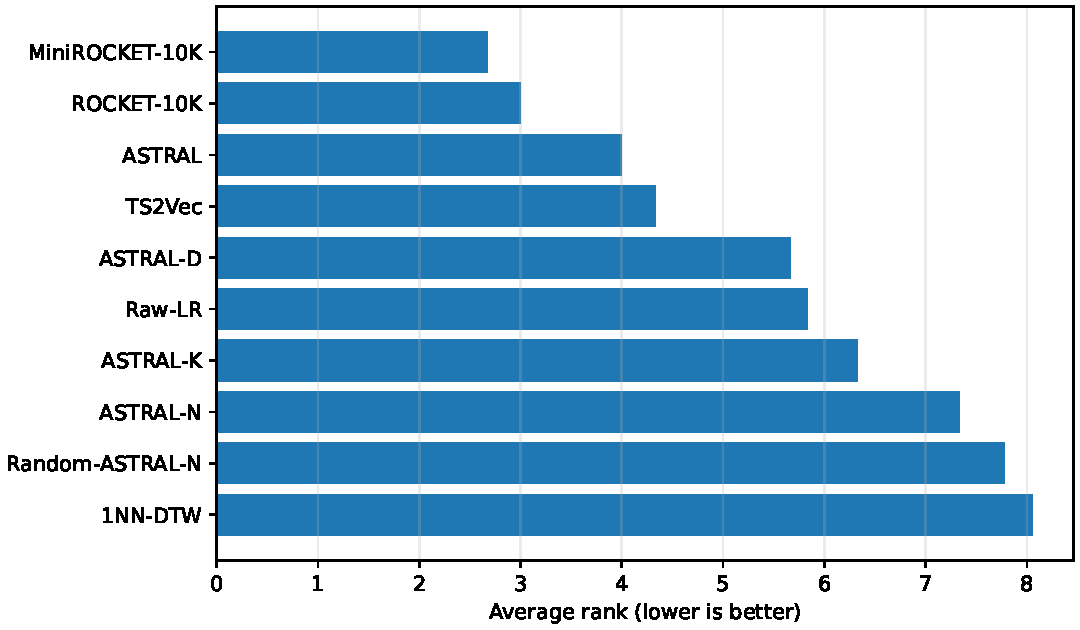
\includegraphics[width=0.85\linewidth]{Fig3.pdf}
		\caption{Average-rank profile for the leading references and the matched neural-only realization. Mean accuracy is reported separately in Table~\ref{tab:mainresults}.}
		\label{fig:ranks}
	\end{figure}
	
	The omnibus null of identical ranks is rejected (Friedman $p=5.00\times10^{-5}$; Iman--Davenport $p=1.89\times10^{-6}$). This result establishes heterogeneity somewhere among the ten methods but does not by itself identify a superior pair. The matched ASTRAL--ASTRAL-N contrast is positive on all nine datasets, with a mean gain of 4.23 percentage points (two-sided Wilcoxon $p=0.0039$, rank-biserial $r_{\mathrm{rb}}=1.00$; unadjusted descriptive values). In contrast, the small mean differences between ASTRAL and TS2Vec or ROCKET-10K do not support a practical superiority claim. Figure~\ref{fig:ranks} and Table~\ref{tab:mainresults} therefore support competitive performance together with evidence for the hybrid mechanism, not universal dominance.
	
	\subsection{Mechanism, label efficiency, and robustness}
	
	Beyond the neural-only contrast reported above, ASTRAL exceeds the teacher-descriptor and complete analytic-only paths by 2.92 and 2.44 points, respectively. Removing pooled shape, teacher descriptors, or energy balancing reduces the mean by 0.40, 0.81, and 1.23 points. Replacing the analytic block with dimension-matched independent noise incurs a 5.56-point loss, so dimensionality alone does not explain the gain. A pooled-input random projection nevertheless comes within 0.23 points of ASTRAL and wins on two datasets, showing that direct morphology is useful without establishing uniqueness of the designed descriptors.
	
	The candidate-objective study identifies residual-dynamics alignment and reliable-order alignment as the largest contributors on the discovery panel. A candidate objective included an additional variance regularizer; removing it improves the four-dataset discovery mean by 1.54 points. The removal is frozen before evaluation on five untouched confirmation datasets and yields a mean effect of $+1.57$ points, with three wins, one tie, and one loss. Accordingly, the variance regularizer is not part of the retained objective in Equation~\eqref{eq:objective}. The loss on AtrialFibrillation shows that the change is beneficial on average rather than uniformly.
	
	ASTRAL is the strongest member of its own family at every evaluated label budget. Its unweighted mean accuracies are 66.94\%, 73.89\%, 75.90\%, and 80.35\% when the probe receives 10\%, 25\%, 50\%, and 100\% of the training labels, respectively. ROCKET-10K has the best rank at the first three budgets, whereas MiniROCKET-10K leads with all labels. Figure~\ref{fig:budget} plots only ASTRAL's four verified means so that the comparative ranks are not approximated graphically.
	
	\begin{figure}[htbp]
		\centering
		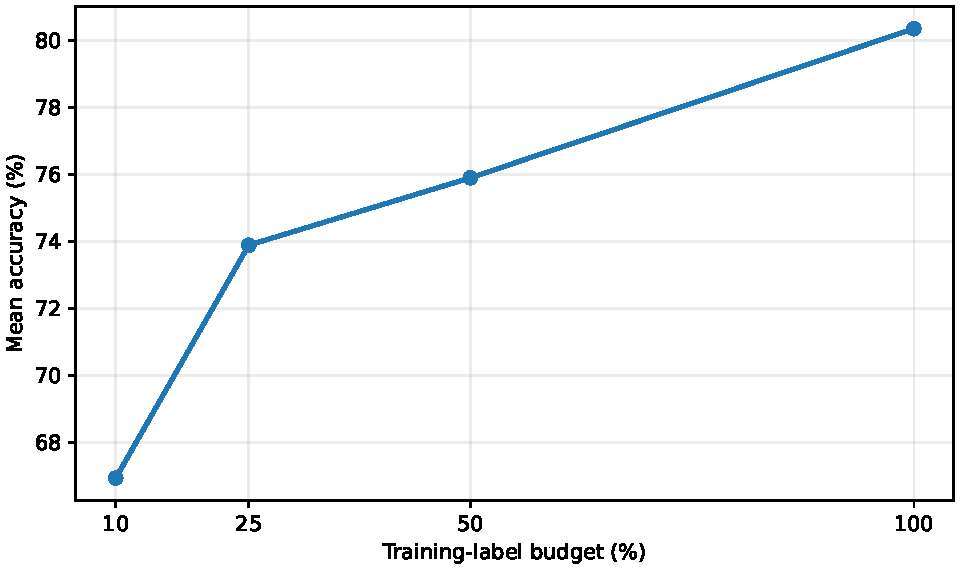
\includegraphics[width=0.80\linewidth]{Fig4.pdf}
		\caption{ASTRAL mean accuracy under four label budgets. Each dataset value first averages five labeled subsets; the plotted value then averages the nine datasets equally.}
		\label{fig:budget}
	\end{figure}
	
	The empirical geometry audit complements the predictive results. The rank-96 spectral tail is zero on seven datasets, 2.48\% on ECG200, and 21.09\% on Epilepsy, instantiating the unavoidable truncation term in Theorem~\ref{thm:decomp}. Training-only kernel--target alignment has a positive but inconclusive dataset-level association with ASTRAL test accuracy (Spearman $\rho=0.60$, $p=0.0876$). The within-minus-between teacher-similarity gap is near zero or negative on AtrialFibrillation and StandWalkJump, consistent with weak performance on those datasets. These diagnostics separate student fidelity from teacher--class alignment; centered kernel alignment is used only for post-hoc diagnosis \cite{cristianini2002alignment}.
	
	Under Gaussian jitter with $\sigma=0.01$, the mean absolute train--test teacher-kernel change is 0.0051, while mean accuracy changes from 80.35\% to 80.71\%. At $\sigma=0.05$ and $0.10$, the kernel changes increase to 0.0328 and 0.0605, and accuracy declines to 73.45\% and 66.91\%, respectively. The small-noise result is consistent with the local continuity statement in Proposition~\ref{prop:teacherstab}; the larger-noise results also show why that proposition must not be interpreted as arbitrary-noise invariance.
	
	\subsection{Scope and limitations}
	
	The guarantees validate the specified geometry and its realizations; task relevance remains empirical. Weak within-class separation on AtrialFibrillation and StandWalkJump illustrates why faithful teacher reproduction need not imply accurate classification. The nine-dataset panel also has limited power for small cross-method differences, and TS2Vec represents rather than exhausts self-supervised encoders. Further boundaries are the contribution of pooled morphology revealed by the random-projection control, potentially task-misaligned fixed component weights, equal-length input requirements, and the quadratic training-set storage of ASTRAL-K. The supported claim is therefore a testable structural mechanism with competitive performance on this panel.

	\section{Conclusion}
	
	ASTRAL defines an auditable trend--residual--spectrum relation, decomposes it at pair level, and realizes it through exact kernel coordinates and an inductive encoder. Finite-sample results characterize kernel validity, attribution, approximation, and fusion, while matched experiments test their classification relevance. Across nine archive datasets, the hybrid consistently improves over its neural-only counterpart and remains competitive with TS2Vec and random-convolution classifiers; alignment diagnostics identify where the structural teacher is weak. Broader benchmarks, variable-length inputs, and identifiable data-adaptive component weights are natural extensions.

\backmatter

\section*{Data availability}

The nine benchmark datasets are publicly available from the UCR and UEA Time Series Classification Archives at \url{https://www.timeseriesclassification.com/}; the official predefined training and test files were used without resplitting. A no-login repository at \url{https://github.com/HanZhang457/ASTRAL-Reproducibility} provides the executable reference implementation, frozen configuration and dependencies, exact downloaded archives, split-file digests, data reconstruction and validation scripts, manuscript sources, and machine-readable validation receipts. Historical row-level ledgers underlying the transcribed numerical summary tables are not part of the current rebuild; those tables are therefore marked fail-closed in the repository until the registered ledgers are restored or the full experiment is rerun.

\section*{Acknowledgements}

This work was supported by the Basic Research Project for Higher Education Institutions of the Educational Department of Liaoning Province (LJ212510173008).

\bibliography{references}

\end{document}
